\section{Reactors}

The governing equations of reactor models implemented in Omnisoot are briefly presented in the following sections. The control volume encompasses the gas mixture and soot particles, as illustrated in Figure~\ref{fig:reactors}. The equations ensure conservation of total mass and energy of the gas and particle system, which can also receive or lose heat through the reactor walls.



\begin{figure}[H]
	\centering
	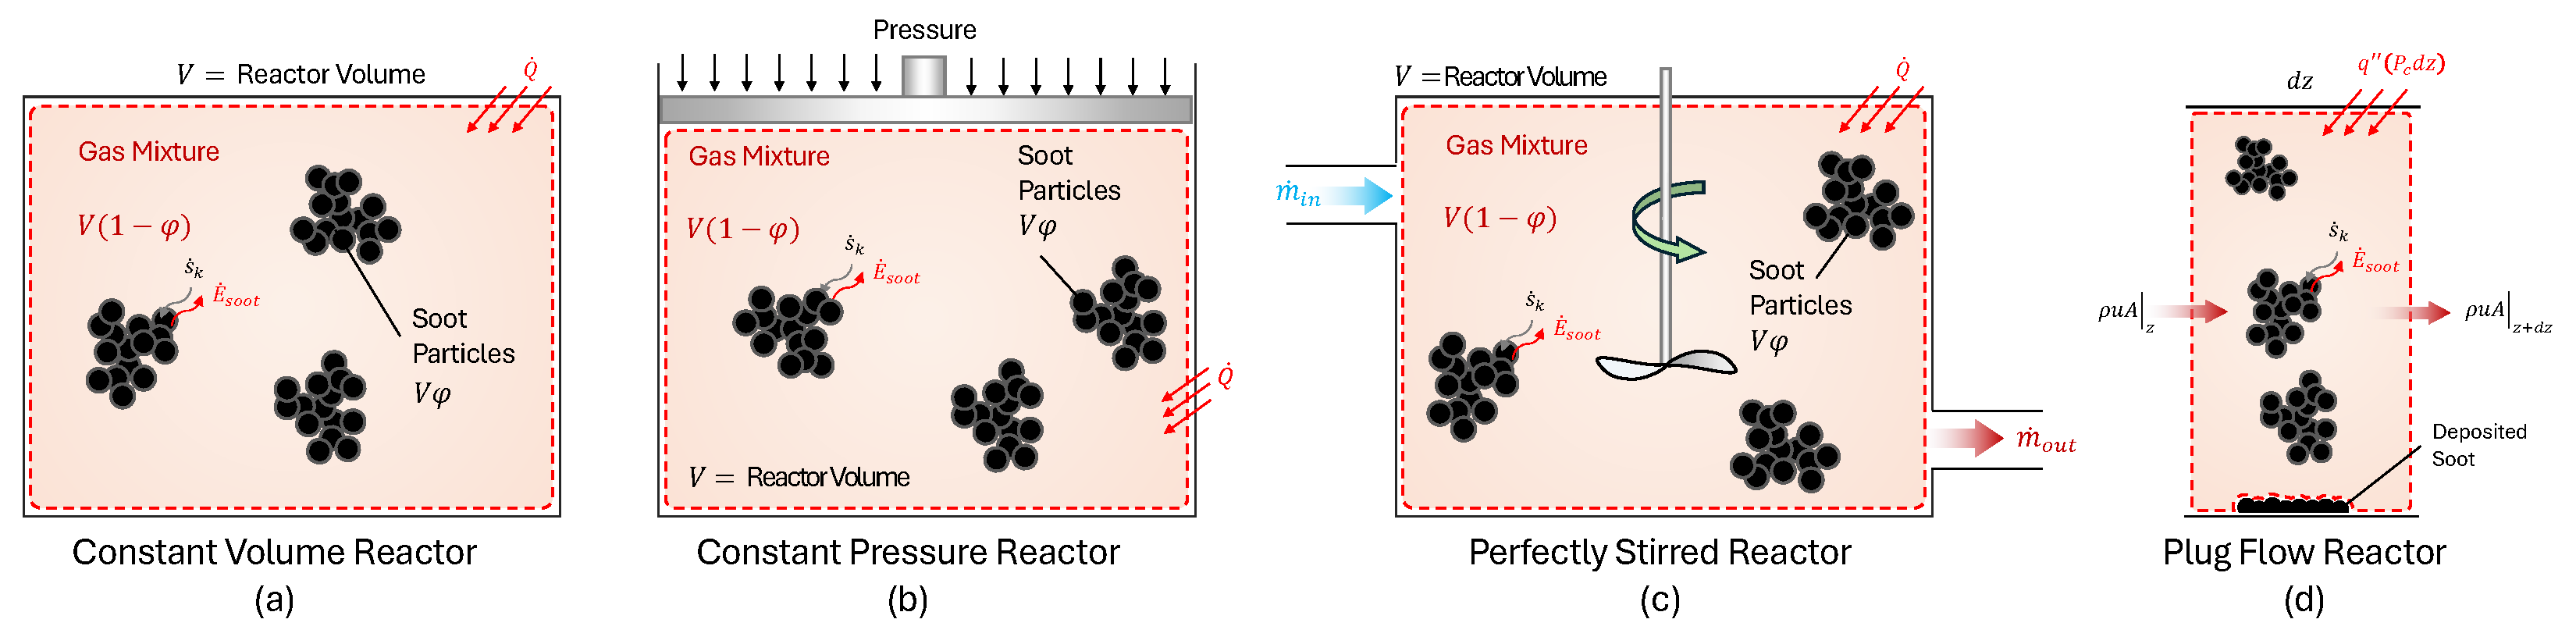
\includegraphics[width=1\textwidth]{Figures/Theory/reactors.pdf}
	\caption{The schematics of constant volume reactor (a), constant pressure reactor (b) perfectly stirred reactor (c), and plug flow reactor (d)}
	\label{fig:reactors} 
\end{figure}


\subsection{Constant Volume Reactor (CVR)}
\label{sec:cvr}
As shown in Figure~\ref{fig:reactors}a, CVR represents a closed system constant volume where chemical reactions converts part of the gas mixture to soot particles. The mass balance equation is written as:

\begin{equation}
	\frac{\mathrm{d}}{\mathrm{d}t}(m) = (1-\varphi)V \sum_i \dot s_i W_i,
	\label{eqn:contconstuv}
\end{equation} 

\noindent where $m$ is the mass of the gas mixture. The rate of change of $m$ is equal to the rate of production of soot mass.
Similarly, the species equation for species $k$ is expressed as:

\begin{equation}
	\frac{\mathrm{d}Y_k}{\mathrm{d}t}
	=
	\frac{1}{\rho}
	\left(
	{\dot{\omega}}_k
	+
	{\dot{s}}_k
	\right)W_k
	-\frac{1}{\rho}Y_k\sum_{i}{{\dot{s}}_i W_i}
	\label{eqn:speciesconstuv}.
\end{equation}

The transport equation for a generic soot variable, $\psi$, can be written as:
\begin{equation}
	\frac{\mathrm{d} \psi}{\mathrm{d} t}= S_{\psi} - \frac{\psi}{\rho} \sum_i \dot{s}_i W_i
	\label{eqn:sootconstuv}.
\end{equation}

The second term on RHS of Equations~\eqref{eqn:speciesconstuv} and~\eqref{eqn:sootconstuv} denotes the change in $Y_k$ and $\psi$, respectively, due to the removal or addition of gas mass by soot-related processes.
The energy conservation for the gas mixture is written in terms of the rate of change of temperature. An external heat source of $\mathrm{\dot{Q}}$ is considered to account for possible heat loss/gain of the reactor.
\begin{equation}
	\begin{split}
		\frac{\mathrm{d} T}{\mathrm{d} t}=
		\frac{1}{\rho c_v+\rho_{soot}f_v c_{soot}}
		\left[
		-\sum_k e_k
		\left(
		\dot{\omega}_k+\dot{s}_k
		\right) W_k
		\right. \\
		\left.
		+e_{soot}\sum_k \dot{s}_k W_k
		+\frac{\dot{Q}}{V(1-\varphi)}
		\right],
	\end{split}
	\label{eqn:energyconstuv}
\end{equation}

\noindent where $\rho_{soot}f_v c_{soot}$ and $e_{soot}\sum_k \dot{s}_k W_k$ represent the formation and sensible energy of soot, respectively. We investigated the effect of considering soot formation and sensible energy on gas and soot properties by simulating the pyrolysis of 30\%~$\mathrm{CH_4}$-Ar with and without considering the above mentioned term. As shown in Figure~\ref{fig:sseeffect}a, neglecting soot sensible energy results in the overprediction of temperature by nearly 150 K and mobility diameter by a factor of 3 during the 80 ms of the simulation. The overprediction of temperature changes gas chemistry, leading to a noticeable decrease in the residual methane and benzene (Figure~\ref{fig:sseeffect}b).



\begin{figure}[H]
	\centering
	\begin{subfigure}[t]{0.43\textwidth}
		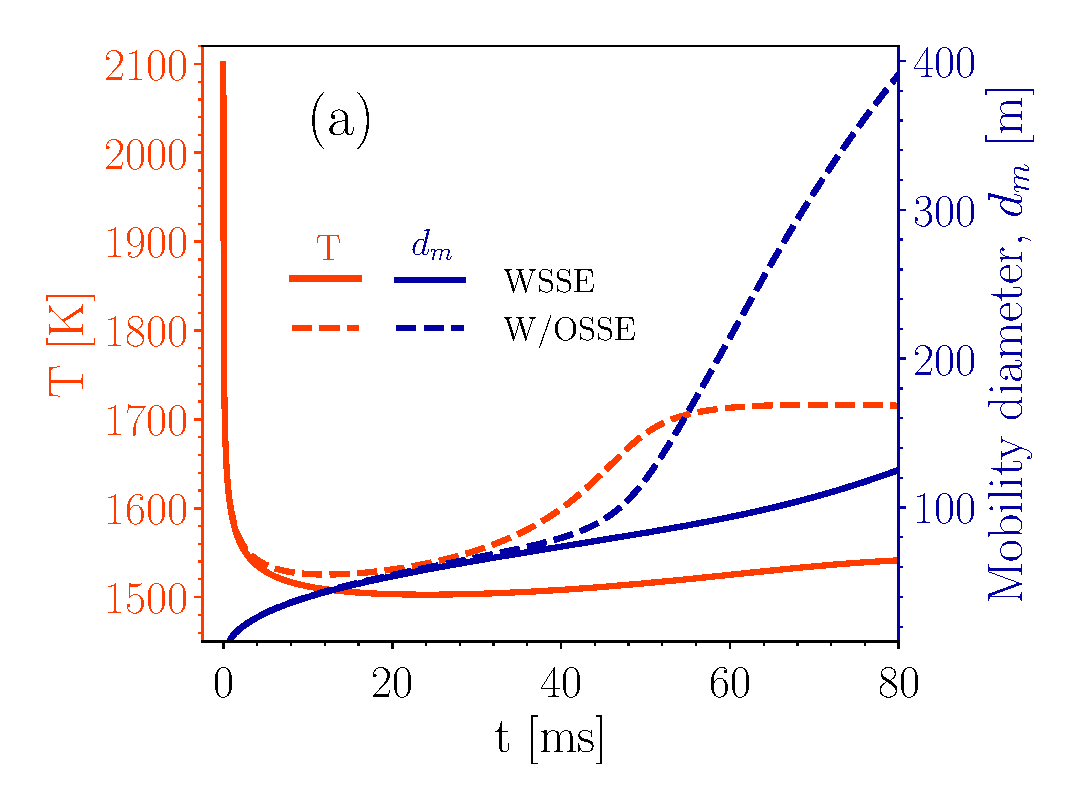
\includegraphics[width=1\textwidth]{Figures/Theory/sse_temp_dm.pdf}
	\end{subfigure}
	\begin{subfigure}[t]{0.4\textwidth}
		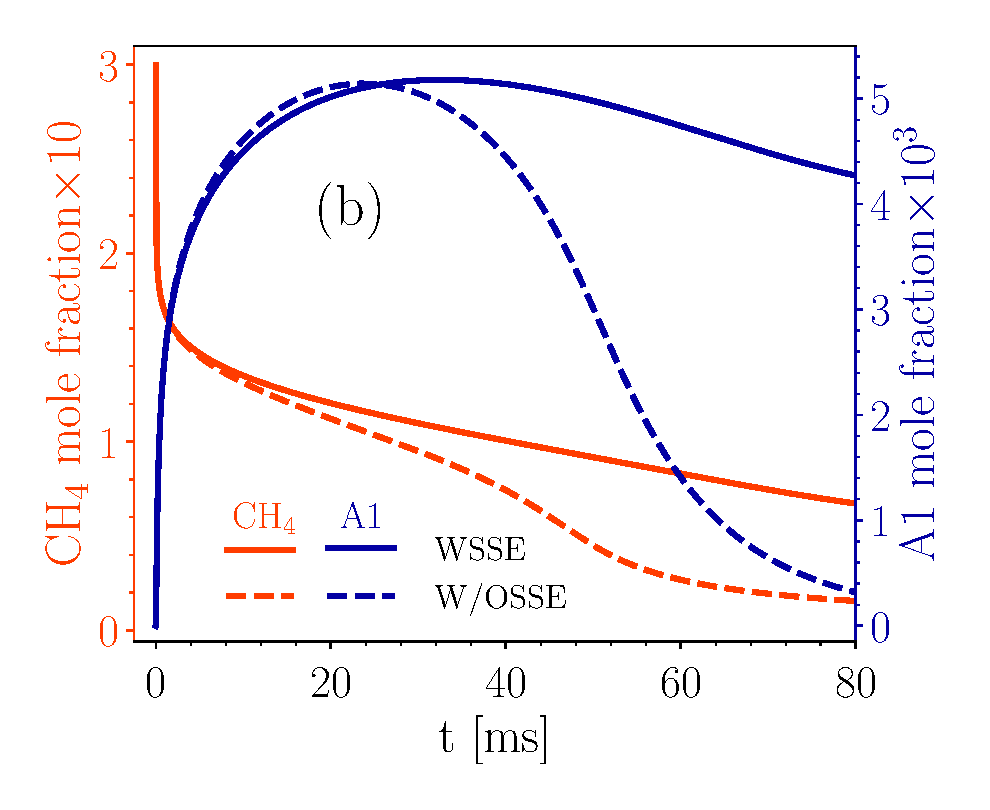
\includegraphics[width=1\textwidth]{Figures/Theory/sse_gasresid.pdf}
	\end{subfigure}
	\caption{The comparison of temperature and soot mobility diameter, $d_m$ (a) and the mole fraction of methane, $\mathrm{CH_4}$, and benzene, A1 in the simulation of the pyrolysis of 30\%$\mathrm{CH_4}$-Ar when soot sensible energy is considered (labeled as ``WSSE") and neglected (labeled as ``W/OSSE"). The CVR is used along with Caltech mechanism~\citep{blanquart2009chemical}, Reactive Dimerization and MPBM}
	\label{fig:sseeffect}
\end{figure}

\subsection{Imposed Pressure Reactor}

As show in Figure~\ref{fig:reactors}b, this reactor is a closed system similar to CVR with a main difference that the boundary can move and change the volume of the system due to an external pressure that can stay constant or vary with time. In either case, the pressure is known a priori in this model. The heat transfer can occur through reactor walls, which changes the internal energy of the gas-particle system.

The equations of mass, species, and soot variables in CPR are the same as those in CVR, but the energy equation is written based on enthalpy, $h$, instead of internal energy, $e$, as:

\begin{equation}
	\begin{split}
		\frac{\mathrm{d} T}{\mathrm{d} t}=
		\frac{1}{\rho c_p+\rho_{soot}f_v c_{soot}}
		\left[
		-\sum_k h_k
		\left(
		\dot{\omega}_k+\dot{s}_k
		\right) W_k \right. \\
		\left.
		+h_{soot}\sum_k \dot{s}_k W_k
		+\frac{\mathrm{d}P}{\mathrm{d}t}
		+\frac{\dot{Q}}{V(1-\varphi)}
		\right]
		\label{eqn:energypressure}.
	\end{split}
\end{equation}


\noindent where $\mathrm{d}P/\mathrm{d}t$ represents the effect of variable pressure on the gas temperature, which is zero when the pressure is constant throughout the process.


\subsection{Perfectly Stirred Reactor (PSR)}
In this reactor, gas enters with a mass flow rate, composition, and temperature of $\dot{m}_{in}$, $Y_{in}$, and $T_{in}$, respectively, and homogeneously reacts with the mixture inside the reactor. The reacting gas reaches a spatially uniform temperature and composition described by $T$ and $Y$. It is assumed that temperature, composition and soot properties of the outflow are the same as the mixture inside reactor. Without soot formation, the inlet and outlet mass flow rates are equal (i.e. ${\dot{m}_{in}}={\dot{m}_{out}}$), but when soot is formed, ${\dot{m}_{out}}$ is slightly less than ${\dot{m}_{in}}$. The nominal residence time of PSR is calculated as:

\begin{equation}
	\tau_{psr} = \frac{\rho V}{\dot{m}_{in}}
	\label{eqn:taupsr}.
\end{equation} 

The conservation of mass of PSR can be written by considering the mass flux of in- and outflow, and the removal of mass due to soot formation as:

\begin{equation}
	\frac{\mathrm{d} m}{\mathrm{d} t}
	=
	\dot{m}_{in} - \dot{m}_{out} 
	+ V(1 - \varphi)\sum_i \dot{s}_i W_i 
	\label{eqn:contpsr}.
\end{equation}

Gas composition is obtained by solving the species transport equations as:

\begin{equation}
	\frac{\mathrm{d} Y_k}{\mathrm{d} t}
	=
	\frac{{\dot{m}}_{in}}{\rho V
		\left(1-\varphi\right)}
	\left(Y_{k,in}-Y_k \right)+
	\frac{1}{\rho}\left[\left(\dot{\omega}_k+\dot{s}_k\right) W_k-Y_k \sum_i \dot{s}_i W_i\right]
	\label{eqn:speciespsr}.
\end{equation}

The soot transport equations can also be expressed as:
\begin{equation}
	\frac{\mathrm{d}\psi}{\mathrm{d}t}
	=
	\frac{{\dot{m}}_{in}}{\rho V
		\left(1-\varphi\right)}
	\left(\psi_{in}-\psi\right)
	+
	S_{\psi}
	-\frac{1}{\rho}\psi\sum_{i}{{\dot{s}}_i W_i}
	\label{eqn:sootpsr}.
\end{equation}

The energy equation for this reactor is written as:
\begin{equation}
	\begin{split}
		\frac{\mathrm{d}T}{\mathrm{d}t}
		=
		\frac{1}
		{
			\rho c_p+\rho_{soot}c_{p,soot}f_v
		}
		\left[
		\frac{{\dot{m}}_{in}}{V(1 - \varphi)}
		\left(h_{in}-h\right)
		-
		\frac{{\dot{m}}_{in}}{V (1 - \varphi)}\sum_{k}\left(Y_{k,in}-Y_k\right)h_k
		\right.\\
		\left.	
		-
		\sum_{k}{
			\left(
			{\dot{\omega}}_k
			+
			{\dot{s}}_k
			\right) W_k h_k}
		+\sum_{i}{{\dot{s}}_i W_i} h_{soot}+\frac{\dot{Q}}{V(1 - \varphi)}
		\right].
	\end{split}
	\label{eqn:energypsr}
\end{equation}



\subsection{Plug Flow Reactor (PFR)}
\label{sec:pfr}
PFR is an ideal representation of a channel or duct where the temperature, composition, and soot properties of a steady-state one-dimensional flow evolve along the reactor. There is no spatial gradient over cross-section due to strong mixing. The diffusion along reactor is negligible.


The continuity equation for PFR is written as:
\begin{equation}
	\frac{\mathrm{d}\dot{m}}{\mathrm{d}z} =(1-\varphi)A \sum_i \dot s_i W_i
	\label{eqn:contpfr}.
\end{equation}

The momentum equation can also be established as:
\begin{equation}
	u (1-f_v) \sum_i \dot s_i W_i + \rho u (1-\varphi) \frac{\mathrm{d}u}{\mathrm{d}z}
	=-\frac{\mathrm{d}}{\mathrm{d}z}(p(1-\varphi))-\frac{\tau_{w}}{R_H} 
	\label{eqn:momenpfr},
\end{equation}
\noindent where $\tau_w$, and $R_H$ are the wall shear stress and hydraulic radius of the reactor. $\tau_w$ can be determined from the friction factor, $f$, as:
\begin{equation}
	\tau_w = \frac{1}{2}\rho u^2 f, 
	\label{eqn:wallshearpfr}
\end{equation}

\noindent where $f$ can be accurately calculated over the entire range of Reynolds numbers, from laminar to turbulent flow, using the explicit formula provided by \citet{haaland1983simple}:


\begin{equation}
	\frac{1}{f^{1/2}} = -1.8 \mathrm{log}
	\left(
	\frac{6.9}{Re}+
	\left[ \frac{\epsilon/D_H}{3.7} \right]^{1.11}
	\right)
	\label{eqn:fpfr},
\end{equation}
\noindent where $\epsilon$ and ${D_H}$ are the wall roughness and the hydraulic radius of the reactor. The species equation can be expressed as:
\begin{equation}
	\frac{\mathrm{d} Y_k}{\mathrm{d} z}=\frac{1}{\rho u}\left[\left(\dot{\omega}_k+\dot{s}_k\right) W_k-Y_k \sum_i \dot{s}_i W_i\right]
	\label{eqn:speciespfr}.
\end{equation}

The soot transport equations can also be written as:
\begin{equation}
	\frac{\mathrm{d} \psi}{\mathrm{d} z}=
	\frac{S_{\psi}}{u}
	-\frac{\psi}{\rho u}\sum_i \dot{s}_i W_i
	-\frac{4}{D_H}\frac{k^i_{dep}\psi}{u},
	\label{eqn:sootpfr}
\end{equation}
\noindent where $k^i_{dep}$ is the deposition velocity of soot particles of section $i$, which is calculated as:

\begin{equation}
	k_{dep}=
	\frac{Sh\cdot D^i}{D_H},
	\label{eqn:kdep}
\end{equation}

\noindent where $Sh=3.66$ for laminar flows, and it calculated using the Berger and Hau correlation~\citep{berger1977mass} for the turbulent flow as:

\begin{equation}
	Sh=
	0.0165Re^{0.86} Sc^{1/3}
	\label{eqn:shdep}.
\end{equation}

The energy equation can be expressed as:
\begin{equation}
	\begin{split}
		\frac{\mathrm{d} T}{\mathrm{d} z}=
		\frac{1}{\rho u c_p+\rho_{soot} u f_v 	c_{p,soot}}
		\left[
		-\sum_k h_k
		\left(
		\dot{\omega}_k+\dot{s}_k
		\right) W_k
		\right. \\
		\left.
		+h_{soot}\sum_k \dot{s}_k W_k
		+q^{\prime \prime}\frac{P_c}{A}
		\right],
	\end{split}
	\label{eqn:energypfr}
\end{equation}
\noindent where $q^{\prime \prime}$ is the wall heat flux of the reactor.
